Natürliches Mapping bedeutet, dass das Layout der Bedienelemente - 
also in diesem Fall die Scrollrichtung der Maus - mit dem Gerät räumlich übereinstimmt.
Die Bedienung ist somit intuitiver. Es macht Sinn, wenn man mit der Maus 'zu sich' - also nach unten -
scrollt, auch die Seite des Bildschirmes nach unten geht. Beim Macbook kann man die
Scrollrichtung sogar definieren und dort wird sie auch als \textit{Natural} bezeichnet, was 
sehr auf natürliches Mapping hindeutet.

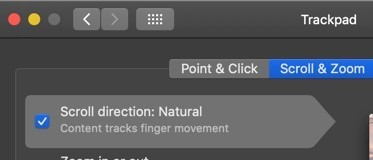
\includegraphics[scale=.5]{images/ScrolldirectionCut.jpg}